\documentclass[11pt]{article}
\usepackage{amsmath}
\usepackage{amssymb}
\usepackage{graphicx}
\usepackage{tabularx}
\usepackage{fancyhdr}
\usepackage{lastpage}

% Page layout
\usepackage[top=1in, bottom=1in, left=1in, right=1in]{geometry}

% Header and footer
\pagestyle{fancy}
\fancyhf{}
\rfoot{Page \thepage}
\renewcommand{\headrulewidth}{0pt}

% Modified Question command with left-aligned number
\newcommand{\questiona}[2]{
    \noindent\textbf{Q#2.} #1 \hfill \textbf{[1 Mark]}
}

\newcommand{\questionb}[2]{
    \noindent\textbf{Q#2.} #1 \hfill \textbf{[2 Marks]}
}

\begin{document}

% Title section with horizontal line
\begin{center}
    \Large\textbf{GATE 2018 - Ecology and Evolution (EY)} \\
    \large\textbf{General Aptitude and Technical Questions} \\
    \rule{\textwidth}{0.5pt} % Horizontal line below heading
\end{center}

\vspace{0.5cm}

% General Aptitude Section
\section*{General Aptitude}

\questiona{Going by the \_\_\_\_\_\_\_ that many hands make light work, the school \_\_\_\_\_ involved all the students in the task.}{1}
\begin{enumerate}
    \item[(A)] principle, principal
    \item[(B)] principal, principle
    \item[(C)] principle, principle
    \item[(D)] principal, principal
\end{enumerate}
\vspace{0.5cm}

\questiona{Her \_\_\_\_\_ should not be confused with miserliness; she is ever willing to assist those in need.}{2}
\begin{enumerate}
    \item[(A)] cleanliness
    \item[(B)] punctuality
    \item[(C)] frugality
    \item[(D)] greatness
\end{enumerate}
\vspace{0.5cm}

\questiona{Seven machines take 7 minutes to make 7 identical toys. At the same rate, how many minutes would it take for 100 machines to make 100 toys?}{3}
\begin{enumerate}
    \item[(A)] 1
    \item[(B)] 7
    \item[(C)] 100
    \item[(D)] 700
\end{enumerate}
\vspace{0.5cm}

\questiona{A rectangle becomes a square when its length and breadth are reduced by 10 m and 5 m, respectively. During this process, the rectangle loses 650 m\(^2\) of area. What is the area of the original rectangle in square meters?}{4}
\begin{enumerate}
    \item[(A)] 1125
    \item[(B)] 2250
    \item[(C)] 2924
    \item[(D)] 4500
\end{enumerate}
\vspace{0.5cm}

\questiona{A number consists of two digits. The sum of the digits is 9. If 45 is subtracted from the number, its digits are interchanged. What is the number?}{5}
\begin{enumerate}
    \item[(A)] 63
    \item[(B)] 72
    \item[(C)] 81
    \item[(D)] 90
\end{enumerate}
\vspace{0.5cm}

\questionb{For integers \(a\), \(b\) and \(c\), what would be the minimum and maximum values respectively of \(a + b + c\) if \(\log |a| + \log |b| + \log |c| = 0\)?}{6}
\begin{enumerate}
    \item[(A)] -3 and 3
    \item[(B)] -1 and 1
    \item[(C)] -1 and 3
    \item[(D)] 1 and 3
\end{enumerate}
\vspace{0.5cm}

\questionb{Given that \(a\) and \(b\) are integers and \(a + a^2b^3\) is odd, which one of the following statements is correct?}{7}
\begin{enumerate}
    \item[(A)] \(a\) and \(b\) are both odd
    \item[(B)] \(a\) and \(b\) are both even
    \item[(C)] \(a\) is even and \(b\) is odd
    \item[(D)] \(a\) is odd and \(b\) is even
\end{enumerate}
\vspace{0.5cm}

\questionb{From the time the front of a train enters a platform, it takes 25 seconds for the back of the train to leave the platform, while travelling at a constant speed of 54 km/h. At the same speed, it takes 14 seconds to pass a man running at 9 km/h in the same direction as the train. What is the length of the train and that of the platform in meters, respectively?}{8}
\begin{enumerate}
    \item[(A)] 210 and 140
    \item[(B)] 162.5 and 187.5
    \item[(C)] 245 and 130
    \item[(D)] 175 and 200
\end{enumerate}
\vspace{0.5cm}

\questionb{Which of the following functions describe the graph shown in the below figure?}{9}

\begin{center}
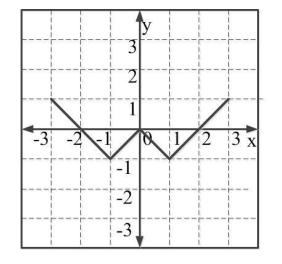
\includegraphics[width=0.5\textwidth]{figures/9}
\end{center}

\begin{enumerate}
    \item[(A)] \( y = ||x| + 1| - 2 \)
    \item[(B)] \( y = ||x| - 1| - 1 \)
    \item[(C)] \( y = ||x| + 1| - 1 \)
    \item[(D)] \( y = ||x - 1| - 1| \)
\end{enumerate}
\vspace{0.5cm}

\questionb{Consider the following three statements: \\
(i) Some roses are red. \\
(ii) All red flowers fade quickly. \\
(iii) Some roses fade quickly. \\
Which of the following statements can be logically inferred from the above statements?}{10}
\begin{enumerate}
    \item[(A)] If (i) is true and (ii) is false, then (iii) is false.
    \item[(B)] If (i) is true and (ii) is false, then (iii) is true.
    \item[(C)] If (i) and (ii) are true, then (iii) is true.
    \item[(D)] If (i) and (ii) are false, then (iii) is false.
\end{enumerate}
\vspace{0.5cm}

\section*{Technical Section}

\questiona{During the Pleistocene, which of the following groups experienced the largest mass extinction?}{1}
\begin{enumerate}
    \item[(A)] Large dinosaurs
    \item[(B)] Large mammals
    \item[(C)] Reptiles
    \item[(D)] Trilobites
\end{enumerate}
\vspace{0.5cm}

\questiona{In group living species, the term ``dilution effect'' refers to}{2}
\begin{enumerate}
    \item[(A)] reduction in aggression among individuals with increasing group size
    \item[(B)] reduction in the mobility of individuals with increasing group size
    \item[(C)] reduction in the reproductive success of individuals with increasing group size
    \item[(D)] reduction in the risk of predation of individuals with increasing group size
\end{enumerate}
\vspace{0.5cm}

\questiona{Which of the following diversity indices best captures species turnover across habitats?}{3}
\begin{enumerate}
    \item[(A)] \( \alpha \)
    \item[(B)] \( \beta \)
    \item[(C)] \( \gamma \)
    \item[(D)] \( \delta \)
\end{enumerate}
\vspace{0.5cm}

\questiona{A duck egg is removed from its mother’s nest and incubated by a barnyard hen. The duckling hatches out in the presence of the barnyard hen and stays in her nest. After a couple of days, the duckling is presented with a choice between its biological mother and the hen that incubated it. The duckling approaches and follows the hen. This set of observations demonstrates the phenomenon of}{4}
\begin{enumerate}
    \item[(A)] habituation
    \item[(B)] imprinting
    \item[(C)] instinct
    \item[(D)] sensitization
\end{enumerate}
\vspace{0.5cm}

\questiona{If both of your ears were located next to each other in the middle of your face, you would have difficulty in resolving the}{5}
\begin{enumerate}
    \item[(A)] direction of a sound
    \item[(B)] duration of a sound
    \item[(C)] loudness of a sound
    \item[(D)] pitch of a sound
\end{enumerate}
\vspace{0.5cm}

\questiona{Forager bees communicate the distance of a food source using a waggle dance upon return to the hive. It is observed that the number of waggles of a dance increases linearly with the distance to the food source. This tells us that the}{6}
\begin{enumerate}
    \item[(A)] number of waggles and distance to food source is negatively correlated
    \item[(B)] number of waggles and distance to food source is positively correlated
    \item[(C)] number of waggles affects the distance to the food source
    \item[(D)] number of waggles and the distance to the food source are uncorrelated
\end{enumerate}
\vspace{0.5cm}

\questiona{Male frogs display to females by producing loud acoustic signals. The use of these signals by bats to locate frogs and prey upon them is an example of}{7}
\begin{enumerate}
    \item[(A)] aposematism
    \item[(B)] deception
    \item[(C)] eavesdropping
    \item[(D)] mimicry
\end{enumerate}
\vspace{0.5cm}

\questiona{A non-venomous, non-toxic species of snake is brightly coloured and closely resembles a venomous snake species in the same habitat. This is most likely a case of}{8}
\begin{enumerate}
    \item[(A)] aggressive mimicry
    \item[(B)] Batesian mimicry
    \item[(C)] masquerade
    \item[(D)] Müllerian mimicry
\end{enumerate}
\vspace{0.5cm}

\questiona{The value of the resting membrane potential of a typical neuron is closest to the equilibrium potential of which of the following ions?}{9}
\begin{enumerate}
    \item[(A)] Ca\(^{++}\)
    \item[(B)] K\(^{+}\)
    \item[(C)] Mg\(^{++}\)
    \item[(D)] Na\(^{+}\)
\end{enumerate}
\vspace{0.5cm}

\questiona{A plant species found in India produces flowers that are white, fragrant, and tubular. Which of the following is the most likely pollinating agent?}{10}
\begin{enumerate}
    \item[(A)] Hummingbirds
    \item[(B)] Lorises
    \item[(C)] Moths
    \item[(D)] Wind
\end{enumerate}
\vspace{0.5cm}

\questiona{Which of the following can be used to test differences between mean tree heights in a tropical versus a temperate forest?}{11}
\begin{enumerate}
    \item[(A)] Binomial test
    \item[(B)] Linear regression
    \item[(C)] Pearson’s correlation
    \item[(D)] Student’s t-test
\end{enumerate}
\vspace{0.5cm}

\questiona{For a species, assuming a relatively short time scale and no evolution, increased interspecific competition will result in a}{12}
\begin{enumerate}
    \item[(A)] larger fundamental niche
    \item[(B)] larger realized niche
    \item[(C)] smaller fundamental niche
    \item[(D)] smaller realized niche
\end{enumerate}
\vspace{0.5cm}

\questiona{In which of the following mating systems is sperm competition likely to evolve?}{13}
\begin{enumerate}
    \item[(A)] Monoandry
    \item[(B)] Monogamy
    \item[(C)] Polyandry
    \item[(D)] Polygyny
\end{enumerate}
\vspace{0.5cm}

\questiona{Copies of genes that arrive in a particular genome by horizontal gene transfer are known as}{14}
\begin{enumerate}
    \item[(A)] analogs
    \item[(B)] homologs
    \item[(C)] ohnologs
    \item[(D)] xenologs
\end{enumerate}
\vspace{0.5cm}

\questiona{In which of the following plants is the dominant stage of the life cycle haploid?}{15}
\begin{enumerate}
    \item[(A)] Cycads
    \item[(B)] Ferns
    \item[(C)] Gymnosperms
    \item[(D)] Mosses
\end{enumerate}
\vspace{0.5cm}

\questiona{Which of the following is NOT typically a characteristic of early successional pioneer plants relative to late successional plants in a tropical rain forest?}{16}
\begin{enumerate}
    \item[(A)] Higher shade tolerance
    \item[(B)] Smaller seed size
    \item[(C)] Smaller size at maturity
    \item[(D)] Wind dispersed seeds
\end{enumerate}
\vspace{0.5cm}

\questiona{Natural populations often deviate from Hardy-Weinberg equilibrium. One possible reason for this is}{17}
\begin{enumerate}
    \item[(A)] no migration
    \item[(B)] no selection
    \item[(C)] random mating
    \item[(D)] small population sizes
\end{enumerate}
\vspace{0.5cm}

\questiona{Which of the following is NOT an example of phenotypic plasticity?}{18}
\begin{enumerate}
    \item[(A)] Density-dependent swarming behavior in locusts
    \item[(B)] Increase in DDT resistance in mosquitos
    \item[(C)] Seasonal variation in plumage colouration in birds
    \item[(D)] Temperature-dependent sex determination in turtles
\end{enumerate}
\vspace{0.5cm}

\questiona{Which of the following is NOT a characteristic of r-selected species?}{19}
\begin{enumerate}
    \item[(A)] Early sexual maturity
    \item[(B)] High juvenile mortality
    \item[(C)] High parental care
    \item[(D)] Large number of offspring
\end{enumerate}
\vspace{0.5cm}

\questiona{A scientist finds a new species of insect and sends a sample to a museum for confirmation. The curator of the museum designates it as a holotype for the newly identified species and asks the scientist to also provide samples of the opposite sex. This sample of the opposite sex is called the}{20}
\begin{enumerate}
    \item[(A)] allotype
    \item[(B)] isotype
    \item[(C)] karyotype
    \item[(D)] neotype
\end{enumerate}
\vspace{0.5cm}

\questiona{Which of the following is NOT essential for a behavioural trait to evolve by natural selection?}{21}
\begin{enumerate}
    \item[(A)] The behavioural trait differs among individuals
    \item[(B)] The behavioural trait is determined at least in part by genes
    \item[(C)] The behavioural trait influences reproductive success
    \item[(D)] The behavioural trait is determined entirely by genes
\end{enumerate}
\vspace{0.5cm}

\questiona{El Niño Southern Oscillation (ENSO) events have occurred approximately every 3–7 years over the last century. The cause of these ENSO events is related to}{22}
\begin{enumerate}
    \item[(A)] large-scale air-sea interactions in the Pacific Ocean
    \item[(B)] strong monsoon winds in the Indian Ocean
    \item[(C)] the melting of icebergs in the Antarctic Ocean
    \item[(D)] unsustainable overfishing in North Atlantic Ocean
\end{enumerate}
\vspace{0.5cm}

\questiona{If the mean of a sample is 5, and the variance is 25, the PERCENT coefficient of variation is \_\_\_.}{23}
\vspace{0.5cm}

\questiona{Consider a diploid population at Hardy-Weinberg equilibrium. For a locus with two alleles, the frequency of the A1A1 genotype is 0.01. The frequency of heterozygotes A1A2 is \_\_\_ (answer up to 2 decimal places).}{24}
\vspace{0.5cm}

\questiona{In a food chain, the efficiency of transfer of energy from one trophic level to the next is 10\%. The PERCENTAGE of energy that is expected to transfer from the second to the fourth level is \_\_\_.}{25}
\vspace{0.5cm}

\questionb{Which of the following is an adaptation for osmoregulation in freshwater teleost fish?}{26}
\begin{enumerate}
    \item[(A)] Excreting large quantities of dilute urine
    \item[(B)] Excreting large quantities of uric acid
    \item[(C)] Having high concentration of blood urea
    \item[(D)] Excreting large quantities of uracil
\end{enumerate}
\vspace{0.5cm}

\questionb{The latitudinal diversity gradient is defined as the decrease in the number of species from the equator to the poles. This can result from}{27}
\begin{enumerate}
    \item[(A)] greater energy input at the poles
    \item[(B)] greater land mass at the poles
    \item[(C)] greater seasonal variation at the poles
    \item[(D)] greater speciation rates at the poles
\end{enumerate}
\vspace{0.5cm}

\questionb{Identify the graph in which natural selection on beak size is LEAST likely to be occurring? For each of the graphs, the slope of the regression line and the associated p-value is given.}{28}
\begin{center}
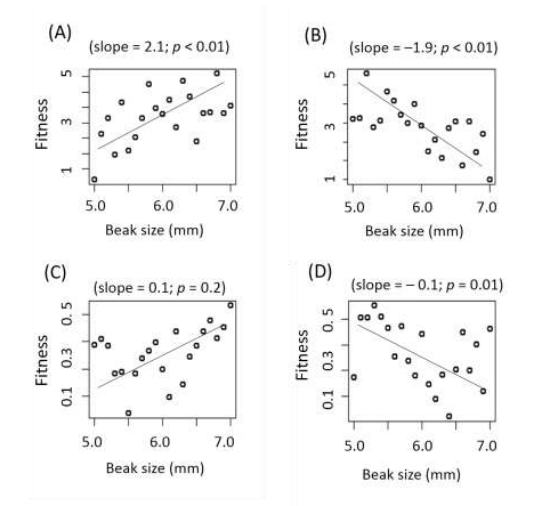
\includegraphics[width=0.7\textwidth]{figures/28}
\end{center}
\vspace{0.5cm}

\questionb{Some species of spiders add additional silk ‘decorations’ to their webs. It is hypothesized that these decorations serve either to lure flies (prey) or to decrease bird (predator) attacks on the spiders. The appropriate way to test these hypotheses would be to compare numbers of}{29}
\begin{enumerate}
    \item[(A)] predators and prey approaching decorated webs
    \item[(B)] predators and prey approaching undecorated webs
    \item[(C)] predators approaching decorated webs with prey approaching undecorated webs
    \item[(D)] predators and prey approaching both decorated and undecorated webs
\end{enumerate}
\vspace{0.5cm}

\questionb{The figure below shows mean annual temperatures (°C) and mean annual precipitation (cm per year) from multiple sites in four regions in India.}{30}
\begin{center}
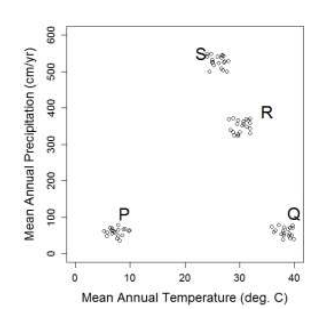
\includegraphics[width=0.5\textwidth]{figures/30}
\end{center}
From this climatic information, we can infer that P, Q, R, and S are LIKELY to be located in:
\begin{enumerate}
    \item[(A)] P: Andaman, Q: Meghalaya, R: Ladakh, S: Rajasthan
    \item[(B)] P: Ladakh, Q: Rajasthan, R: Andaman, S: Meghalaya
    \item[(C)] P: Meghalaya, Q: Ladakh, R: Rajasthan, S: Andaman
    \item[(D)] P: Rajasthan, Q: Andaman, R: Meghalaya, S: Ladakh
\end{enumerate}
\vspace{0.5cm}

\questionb{For a pair of interacting species, increased specialization and decreased niche breadth in both species would result in}{31}
\begin{enumerate}
    \item[(A)] decreased intraspecific competition and increased interspecific competition
    \item[(B)] decreased intraspecific competition and decreased interspecific competition
    \item[(C)] increased intraspecific competition and increased interspecific competition
    \item[(D)] increased intraspecific competition and decreased interspecific competition
\end{enumerate}
\vspace{0.5cm}

\questionb{Males of a bird species provide parental care by feeding nestlings before they fledge. Which of the following is a PROXIMATE explanation for this behaviour?}{32}
\begin{enumerate}
    \item[(A)] Feeding nestlings increases their survivorship after fledging
    \item[(B)] High prolactin levels cause males to feed their nestlings
    \item[(C)] Males from all species in this genus provide parental care
    \item[(D)] Males that provide parental care have higher fitness
\end{enumerate}
\vspace{0.5cm}

\questionb{The courtship display of a spider species consists of both visual and vibrational signals. Females respond to the display by approaching males. In an experiment, females were presented with 3 treatments: i) only videos of displaying males, ii) only vibrational signals of the display, and iii) both videos of displaying males and vibrational signals. The results are given below:

\begin{center}
\begin{tabular}{|c|c|}
\hline
\textbf{Treatment} & \textbf{Percent of responding females} \\
\hline
Videos only & 55\% \\
Vibrational signals only & 0\% \\
Videos plus vibrational signals & 95\% \\
\hline
\end{tabular}
\end{center}

Results from this experiment show that}{33}
\begin{enumerate}
    \item[(A)] vibrational signals are necessary to evoke a response
    \item[(B)] vibrational signals are sufficient to evoke a response
    \item[(C)] visual and vibrational signals are necessary to evoke a response
    \item[(D)] visual signals are necessary to evoke a response
\end{enumerate}
\vspace{0.5cm}

\questionb{Moth ears typically consist of a membranous eardrum backed by an air cavity. Ears in different phylogenetic groups of moths have evolved on different body parts. Moth ears are thus best described as}{34}
\begin{enumerate}
    \item[(A)] convergent organs
    \item[(B)] homologous organs
    \item[(C)] maladaptive organs
    \item[(D)] vestigeal organs
\end{enumerate}
\vspace{0.5cm}

\questionb{Increased anthropogenic disturbance has resulted in an overall decrease in densities of trees and an increase in fragmentation of forests. Which of the following types of trees will have the greatest reduction in reproductive success?}{35}
\begin{enumerate}
    \item[(A)] Dioecious species
    \item[(B)] Monoecious species
    \item[(C)] Self-compatible hermaphrodites
    \item[(D)] Self-incompatible hermaphrodites
\end{enumerate}
\vspace{0.5cm}

\questionb{A study examined the effect of neighbours on plants when grown at low or high altitudes. The researcher measured Relative Neighbour Effect (RNE), defined as: \\ 
RNE = Biomass with neighbours – Biomass without neighbours.}{36}
\begin{center}
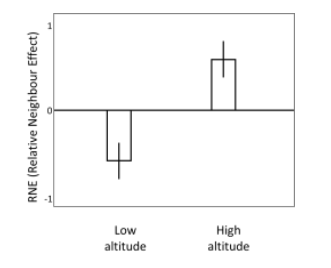
\includegraphics[width=0.5\textwidth]{figures/36}
\end{center}
The results shown above demonstrate
\begin{enumerate}
    \item[(A)] competition at both altitudes
    \item[(B)] competition at high altitudes, and facilitation at low altitudes
    \item[(C)] competition at low altitudes, and facilitation at high altitudes
    \item[(D)] facilitation at both altitudes
\end{enumerate}
\vspace{0.5cm}

\questionb{Match the combination of flora and fauna from the list, to the state where they are found.\\
\textbf{Combination \hspace{1cm} Fauna; Flora}\\
P \hspace{1cm} Red panda; Rhododendron\\
Q \hspace{1cm} Pygmy hog; Elephant grass\\
R \hspace{1cm} Tiger; Mangrove\\
S \hspace{1cm} Hangul; Chinar}{37}
\begin{enumerate}
    \item[(A)] P: Assam; Q: Jammu \& Kashmir; R: West Bengal; S: Sikkim
    \item[(B)] P: Jammu \& Kashmir; Q: Assam; R: West Bengal; S: Sikkim
    \item[(C)] P: Sikkim; Q: Assam; R: West Bengal; S: Jammu \& Kashmir
    \item[(D)] P: Sikkim; Q: West Bengal; R: Assam; S: Jammu \& Kashmir
\end{enumerate}
\vspace{0.5cm}

\questionb{A parent population (P) is split into three daughter populations (Q, R, and S) which grow in three different habitats. After 1000 generations, the equilibrium frequency distribution of a trait in each of the daughter populations is shown in the figure below. For reference, the vertical line represents the mean of the parent population.}{38}
\begin{center}
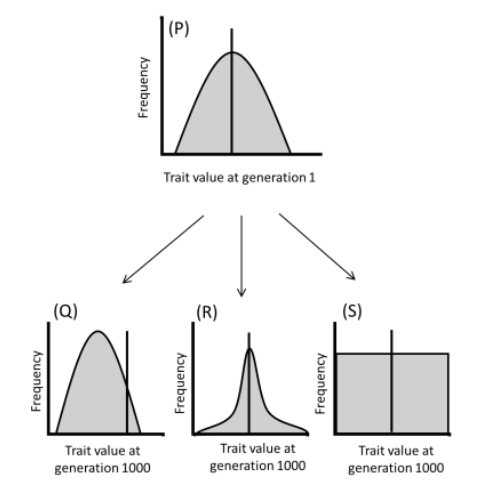
\includegraphics[width=0.5\textwidth]{figures/38}
\end{center}
From this information, one can infer that the subpopulations experienced the following selection regimes:
\begin{enumerate}
    \item[(A)] Q: Directional; R: Stabilizing; S: No selection
    \item[(B)] Q: Directional; R: Stabilizing; S: Stabilizing
    \item[(C)] Q: Directional; R: Directional; S: Stabilizing
    \item[(D)] Q: Stabilizing; R: Directional; S: No selection
\end{enumerate}
\vspace{0.5cm}

\questionb{The character matrix below lists four taxa (P–S) and their nine characters (i–ix). A character state is designated as ‘0’ if it is ancestral and ‘1’ if it is derived. Which of the following phylogenetic trees is obtained by cladistic analysis of these data?}{39}
\begin{center}
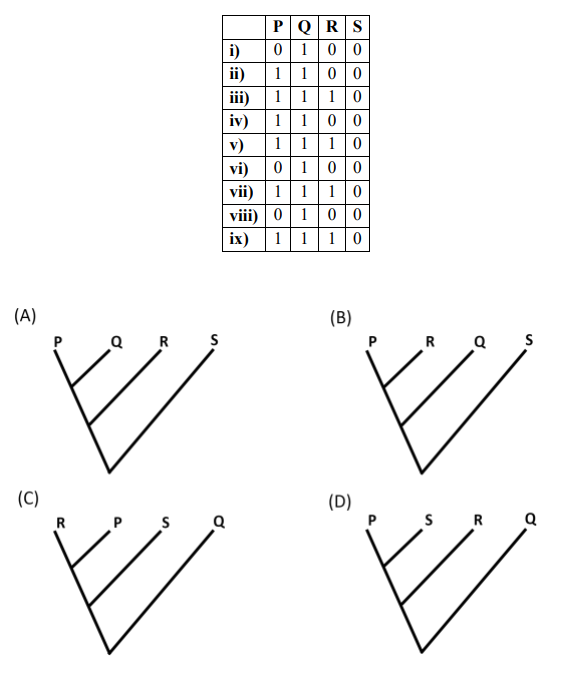
\includegraphics[width=0.8\textwidth]{figures/39}
\end{center}
\vspace{0.5cm}

\questionb{The reactions below (R1 and R2) represent different carbon fixation pathways in photosynthesis.\\
RuBP represents Ribulose bisphosphate.\\
Rubisco represents RuBP carboxylase-oxygenase.\\
PGA represents Phosphoglyceric acid.\\
PEP represents Phosphoenolpyruvate.\\

\textbf{R1.} CO\(_2\) + RuBP \(\xrightarrow{\text{Rubisco}}\) PGA\\
\textbf{R2.} CO\(_2\) + PEP \(\xrightarrow{\text{PEP-Carboxylase}}\) Malic Acid

Which of the following is CORRECT?}{40}
\begin{enumerate}
    \item[(A)] R1 and R2 both occur in C-3 and CAM photosynthesis
    \item[(B)] R1 occurs in C-4 photosynthesis; R2 occurs in C-3 photosynthesis
    \item[(C)] R1 occurs in C-3 photosynthesis; R2 occurs in C-4 photosynthesis
    \item[(D)] R1 occurs in C-4 and CAM photosynthesis; R2 occurs in C-3 photosynthesis
\end{enumerate}
\vspace{0.5cm}

\questionb{A fish species is sexually dimorphic: males possess ultraviolet (UV) spots on their bodies which are lacking in females. Females prefer males with larger and more intense UV spots as mates. Which of the following statements is a plausible reason for the spots being coloured ultraviolet?}{41}
\begin{enumerate}
    \item[(A)] Females assess males from long distances
    \item[(B)] Females are not sensitive to UV light
    \item[(C)] Ultraviolet spots are a poor indicator of male quality
    \item[(D)] Ultraviolet spots are more conspicuous to predators
\end{enumerate}
\vspace{0.5cm}

\questionb{A climate scientist notices a trend in atmospheric CO\(_2\) concentrations (in ppm) at a research station. Although overall CO\(_2\) is rising over decades, there are intra-annual fluctuations, as shown in the figure below.}{42}
\begin{center}
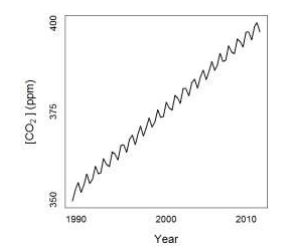
\includegraphics[width=0.5\textwidth]{figures/42}
\end{center}
These fluctuations can be attributed to
\begin{enumerate}
    \item[(A)] burning of fossil fuels by automobiles and industry
    \item[(B)] oscillations due to El Niño and La Niña events
    \item[(C)] rising sea levels due to melting of polar ice-caps
    \item[(D)] seasonal trends in photosynthesis and respiration
\end{enumerate}
\vspace{0.5cm}

\questionb{Four islands differ in size (small = 10 km\(^2\), large = 100 km\(^2\)) and distance from the mainland (near = 50 km, far = 500 km).\\
Island P is small and near the mainland;\\
Island Q is small and far from the mainland;\\
Island R is large and near the mainland;\\
Island S is large and far from the mainland.\\
Let \(N_P\), \(N_Q\), \(N_R\) and \(N_S\) denote the number of species on islands P, Q, R and S, respectively. Which of the following is consistent with the theory of island biogeography?}{43}
\begin{enumerate}
    \item[(A)] \(N_Q > N_S > N_P > N_R\)
    \item[(B)] \(N_R > N_Q > N_P > N_S\)
    \item[(C)] \(N_Q > N_P > N_S > N_R\)
    \item[(D)] \(N_R > N_P > N_S > N_Q\)
\end{enumerate}
\vspace{0.5cm}

\questionb{The rate of population growth (\( \frac{dN}{dt} \)) over time (t) is shown below.}{44}
\begin{center}
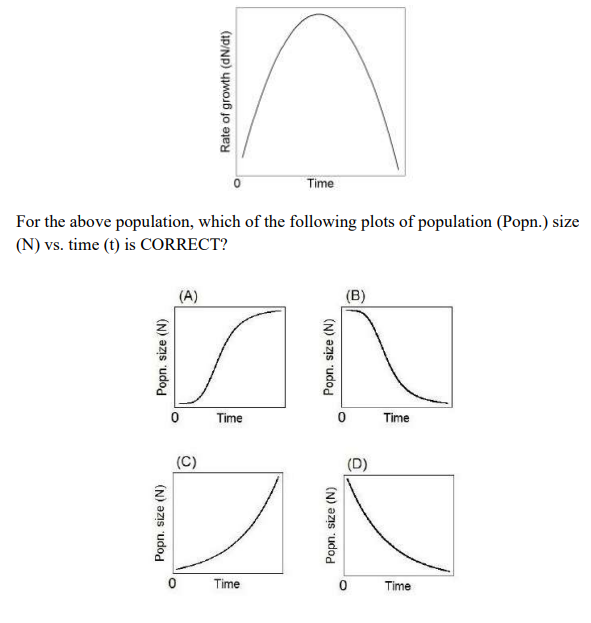
\includegraphics[width=0.8\textwidth]{figures/44}
\end{center}
\vspace{0.5cm}

\questionb{The pedigree below details a late onset genetic disease among humans. Males are represented as squares and females as circles. Individuals with the disease are depicted as black, and those without it are depicted as white. Which of the following best describes the pattern of inheritance of the disease-causing gene?}{45}
\begin{center}
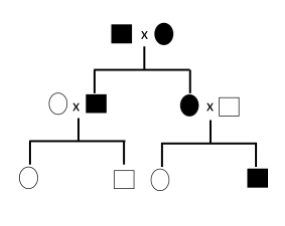
\includegraphics[width=0.5\textwidth]{figures/45}
\end{center}
\begin{enumerate}
    \item[(A)] Mitochondrial
    \item[(B)] X-linked dominant
    \item[(C)] X-linked recessive
    \item[(D)] Y-linked
\end{enumerate}
\vspace{0.5cm}

\questionb{Match the following scientists with the concepts or theories they are associated with.\\
(P) WD Hamilton \hspace{0.5cm} (i) Neutral Theory of Molecular Evolution\\
(Q) RA Fisher \hspace{1.15cm} (ii) Island Biogeography\\
(R) M Kimura \hspace{1.15cm} (iii) Inclusive Fitness\\
(S) RH MacArthur \hspace{0.5cm} (iv) Runaway Sexual Selection}{46}
\begin{enumerate}
    \item[(A)] P-iii, Q-i, R-iv, S-ii
    \item[(B)] P-ii, Q-iii, R-iv, S-i
    \item[(C)] P-iii, Q-iv, R-i, S-ii
    \item[(D)] P-ii, Q-iii, R-i, S-iv
\end{enumerate}
\vspace{0.5cm}

\questionb{Which of the following is an example of complete intrinsic post-zygotic reproductive isolation between two species P and Q?}{47}
\begin{enumerate}
    \item[(A)] P and Q can mate and have fertile offspring
    \item[(B)] P and Q can mate but their offspring are inviable
    \item[(C)] P and Q have breeding seasons during different times of the year
    \item[(D)] P and Q have different courtship behaviour
\end{enumerate}
\vspace{0.5cm}

\questionb{Match the animals to their locomotor adaptation.\\
(P) Volant \hspace{2cm} (i) Ostrich\\
(Q) Fossorial \hspace{1.6cm} (ii) Slow Loris\\
(R) Arboreal \hspace{1.5cm} (iii) Naked Mole Rat\\
(S) Cursorial \hspace{1.5cm} (iv) Bat}{48}
\begin{enumerate}
    \item[(A)] P-iv, Q-i, R-iii, S-ii
    \item[(B)] P-iv, Q-iii, R-ii, S-i
    \item[(C)] P-iii, Q-iv, R-i, S-ii
    \item[(D)] P-ii, Q-iii, R-i, S-ii
\end{enumerate}
\vspace{0.5cm}

\questionb{Paralogs are genes that are the products of gene duplication events within a species. Orthologs are genes in different species that share a common ancestral gene. The figure below describes the evolutionary history of a hypothetical gene X in organism Y. This gene undergoes a duplication event. Later, Y splits into two species Y1 and Y2, and this gives rise to four copies of the gene - P, Q, R and S. Which option best describes the relationships between the four copies of the gene X?}{49}
\begin{center}
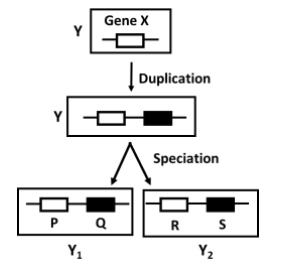
\includegraphics[width=0.5\textwidth]{figures/49}
\end{center}
\begin{enumerate}
    \item[(A)] P \& Q are orthologs, Q \& R are paralogs
    \item[(B)] R \& S are orthologs, S \& Q are paralogs
    \item[(C)] R \& S are orthologs, Q \& R are paralogs
    \item[(D)] P \& R are orthologs, R \& S are paralogs
\end{enumerate}
\vspace{0.5cm}

\questionb{The frequency distribution of beak sizes of a bird species is symmetric but not normally distributed. If the mean value of beak size is 6 mm, standard deviation is 25 mm and kurtosis is 10, then the median is \_\_\_ mm.}{50}
\vspace{0.5cm}

\questionb{An altruist provides help worth 10 units of fitness to a recipient, at a personal cost of 1 unit of fitness. As per kin-selection theory, the minimum value of genetic relatedness between the actors and the recipients that is necessary to maintain altruism in the population is \_\_\_ (answer up to 1 decimal place).}{51}
\vspace{0.5cm}

\questionb{A population grows from a size of 100 individuals at \(t = 0\), to 1000 individuals at \(t = 100\), following density-independent growth. The ratio of per-capita growth rates at the initial (at \(t = 0\)) to the final (at \(t = 100\)) time is \_\_\_.}{52}
\vspace{0.5cm}

\questionb{The probability that a bush has a cricket is 0.1. The probability of a spider being present on a bush is 0.2. When both a spider and a cricket are present on a bush, the probability of encountering each other is 0.2. The probability of a spider consuming a cricket it encounters is 0.5. Assuming that predation only occurs on bushes, the probability that a cricket is preyed on by a spider is \_\_\_ (answer up to 3 decimal places).}{53}
\vspace{0.5cm}

\questionb{A plant produces seeds that can be dispersed by birds or mammals. The probability that a seed is dispersed by a bird is 0.25, and by a mammal is 0.5. The bird can disperse a seed to three patches A, B, or C with a probability 0.5, 0.4 or 0.1, respectively. On the other hand, the mammal disperses a seed to the same patches A, B, or C, with a probability 0.15, 0.8 and 0.05, respectively. The probability that a given seed is dispersed to patch B is \_\_\_ (answer up to 1 decimal place).}{54}
\vspace{0.5cm}

\questionb{The species area relationship of trees in Mudumalai Tiger Reserve is given by \(S = 0.1 \times A^{0.3}\), where \(S\) is the number of species in a given area \(A\). When \(\log S\) is plotted against \(\log A\), the slope of the resulting relationship is \_\_\_ (answer up to 1 decimal place).}{55}
\vspace{0.5cm}

\vspace{5cm}
\begin{center}
\textbf{END OF THE QUESTION PAPER}\\
\rule{\textwidth}{0.5pt}
\end{center}



\end{document}